\chapter{Usability - Tests}
\begin{tiny}
	RS, TF\\
	\ \\
\end{tiny}
Um das \textbf{ofCourse} System bezüglich dem Gesichtspunkt der Benutzbarkeit bzw. der Benutzerfreundlichkeit zu testen,
wurden unvoreingenommene Testpersonen gesucht, welche das System testeten und anschließend das System, aufgrund der
während der Tests gewonnenen Eindrücke evaluierten.\\
\\
Die Usability - Test wurden durchgeführt um die Erfüllung des Punktes {\it Benutzbarkeit} der Qualitätsbestimmungen
aus dem Pflichtenheft, welcher von uns als sehr wichtig eingestuft wurde, zu validieren.

\section{Durchführung}
Für die Durchführung der Test wurden zufällig ausgewählte Personen vom Campus herangezogen. Einziger Gesichtspunkt für die Auswahl der Testpersonen war, dass sie das System ofCourse bisher nicht kannten und auch noch nie damit gearbeitet haben und somit unvoreingenommen an die Test herangingen.\ \\
\ \\
Wenn die angesprochene Person sich für den Test bereit erklärt hatte, wurde sie von uns zufällig einer der Testgruppen zugeordnet und über den Ablauf des Tests aufgeklärt. Die Testpersonen erhielten je nach Gruppe ihre Arbeitsanweisungen und wurden belehrt, dass sie den Test eigenständig und wenn möglich ohne Unterbrechung durchführen sollten. Anschließend sollten die Testpersonen eigenständig die Arbeitsanweisungen ausführen. Fragen der Probanden bezüglich den Aufgaben wurden seitens der Testleiter im Normalfall nicht beantwortet.\\
\ \\
Nach Abschluss des Test wurden die Testpersonen dazu aufgefordert den Feedback - Fragebogen \ref{fig:OfCourseFeedback} auszufüllen.\\
Die Testleiter notierten bei jeder Person die Dauer, welche für die Bearbeitung der Aufgaben benötigt wurde.



\section{Material}
Für die Durchführung der Tests wurden folgende Materialien angefertigt.
\subsection{Testanweisungen}
Für die Durchführung der Test wurden Arbeitsanweisungen für die Testpersonen erstellt. Zum einen mit dem Zweck den Test in einem angemessenen zeitlichen Rahmen durchführbar zu machen, zum anderen um die Vergleichbarkeit der verschiedenen Testdurchläufe zu ermöglichen.\ \\
Es wurden drei verschiedene Arbeitsanweisungen erstellt, nämlich für Testgruppe 1, Testgruppe 2, Testgruppe 3. Die Arbeitsanweisungen\ref{fig:Anweisungen1} der Testgruppe 1 beinhalten Funktionen, welche einem {\it registrierten Benutzer} zur Verfügung stehen und umfassten unter Anderem das Registrieren im System und das Anmelden zu einem Kurs.\\
Die Arbeitsanweisungen\ref{fig:Anweisungen2} der Gruppe 2  beinhalten Funktionen von {\it Kursleitern}, beispielsweise das Bearbeiten eines Kurses bzw. das Anlegen von Kurseinheiten.\\
Die Anweisungen\ref{fig:Anweisungen3} für Testgruppe 3 beinhalten schließlich Funktionen, welche nur dem {\it Administrator} zur Verfügung stehen, wie etwa das Festlegen des Überziehungskredits oder das Erstellen eines Kurses.
\subsection{Fragebogen}
Um die Eindrücke der Testpersonen festzuhalten, wurde ein kurzer Fragebogen erstellt. Dieser ist zweigeteilt. \\
Der erste Teil besteht aus fünf kurzen Aussagen, welche die Testpersonen auf einer Skala von {\it Trifft gar nicht zu} bis 
{\it Trifft voll zu} bewerten sollen. Diese Aussagen beziehen sich auf verschiedene Aspekte der Benutzbarkeit.
Zu diesen zählen unter Anderem die Gestaltung der Oberfläche, die intuitive Bedienbarkeit und das schnelle Auffinden der Funktionen.\\
(vgl. Feedback - Fragebogen ofCourse \ref{fig:OfCourseFeedback} ).\ \\
\ \\
Der zweite Teil des Fragebogens besteht aus offenen Fragen, welche von den Testpersonen kurz zu beantworten sind.\\
Unter Anderem wird dabei gefragt, welcher Aspekt des Systems den Benutzer besonders gut gefallen hat und welche Verbesserungen er sich am System wünschen würde.\\
Zum Schluss des Fragebogens können die Testpersonen unter dem Punkt {\it Meine letzten Worte...} noch einen allgemeinen Kommentar zum System abgeben. \\
(vgl. Feedback - Fragebogen ofCourse \ref{fig:OfCourseFeedback} ).\ \\


\section{Ergebnisse}
Um die Eindrücke der Testpersonen protokollieren und auswerten zu können, wurden sie gebeten einen Fragebogen auszufüllen.
Im Folgenden werden die gewonnenen Ergebnisse anhand der einzelnen Punkte des Fragebogens aufgeführt. Zusätzlich
wurde auch noch die Bearbeitungszeit der Tests erhoben.

\subsection{Frage 1}
\begin{center}
	{\it Ich habe mich in ofCourse schnell zurechtgefunden.}
\end{center}
\begin{figure}[h]
\centering
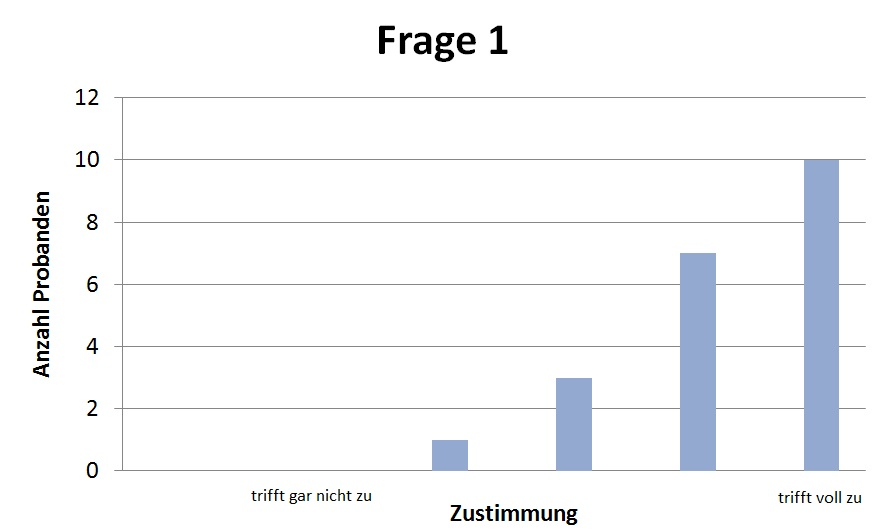
\includegraphics[width=0.7\linewidth]{img/Frage1}
\caption{Gesamtergebnis Frage 1}
\label{fig:Frage1}
\end{figure}
Eine hohe Usability zeichnet sich unter Anderem durch eine intuitive Bedienbarkeit aus, welche sich beispielsweise darin äußert, dass ein Nutzer sich bereits beim ersten Besuch einer Anwendung schnell zurecht findet. Bei den Probanden wurde darauf geachtet, dass diese noch keine Erfahrung im Umgang mit ofCourse haben. Aus den erhobenen Ergebnissen geht hervor, dass sich der Großteil der Testpersonen überwiegend schnell zurechtgefunden haben, was zeigt, dass ofCourse einfach zu bedienen ist, also eine hohe Usability aufweist. Unsere Ergebnisse hier zeigten außerdem eine kleine Abweichung bei den Testgruppen. So fiel es vor allem den normalen Nutzern, also Testgruppe 1, sehr leicht, das System zu benutzen, während es Probanden der Testgruppe 3, die Systemadministratoren, insgesamt als etwas schwerer empfanden.
\newpage
\subsection{Frage 2}
\begin{center}
	{\it ofCourse ist übersichtlich und leicht verständlich.}
\end{center}
\begin{figure}[h]
\centering
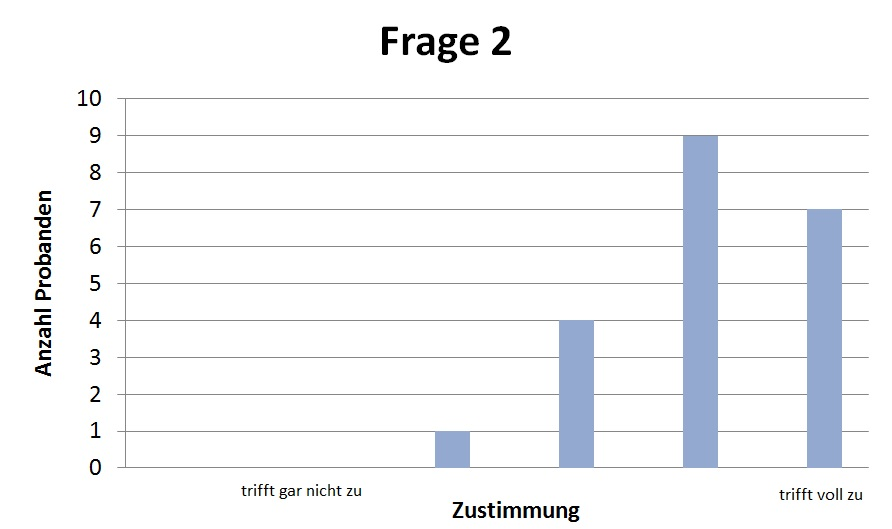
\includegraphics[width=0.7\linewidth]{img/Frage2}
\caption{Gesamtergebnis Frage 2}
\label{fig:Frage2}
\end{figure}
Um als System leicht bedienbar zu sein, ist große Übersichtlichkeit und leichte Verständlichkeit von vornherein notwendig. Wie in Abbildung 3.2 zu erkennen ist, empfand der Großteil der Testpersonen ofCourse als übersichtlich und leicht verständlich. Fast genauso viele stimmten der Aussage voll zu. Dies zeigt, dass der Umgang mit der Webanwendung, bereits in kürzester Zeit und ohne großen Lernaufwand, möglich ist.
\newpage
\subsection{Frage 3}
\begin{center}
	{\it Die gestellten Aufgaben waren mit ofCourse einfach zu lösen.}
\end{center}
\begin{figure}[h]
\centering
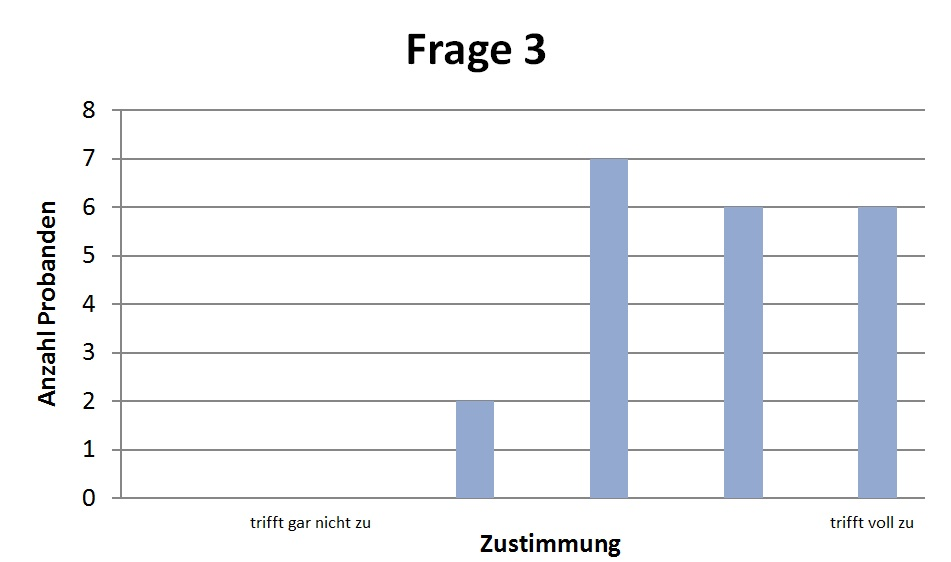
\includegraphics[width=0.7\linewidth]{img/Frage3}
\caption{Gesamtergebnis Frage 3}
\label{fig:Frage3}
\end{figure}
Bei den, an die Testpersonen gestellten, Aufgaben handelt es sich um Standardinteraktionen, welche im laufenden Betrieb sehr häufig getätigt werden. Diese zu lösen muss möglichst einfach und ohne Komplikationen von statten gehen. Die Ergebnisse der Frage 3 zeigen, dass die Aufgaben zu lösen sind, jedoch in manchen Fällen noch nicht unbedingt sehr leicht. Um einer hohen Usability gerecht zu werden, ist hier also an manchen Stellen Nachbesserungsbedarf notwendig. Die Ergebnisse zeigten außerdem, dass unabhängig von den einzelnen Aufgabenbereichen der Testgruppen nachgebessert werden muss, denn die Verteilung der Antworten fiel bei allen dreien sehr ähnlich aus.
\newpage
\subsection{Frage 4}
\begin{center}
	{\it Das Design von ofCourse spricht mich an.}
\end{center}
\begin{figure}[h]
\centering
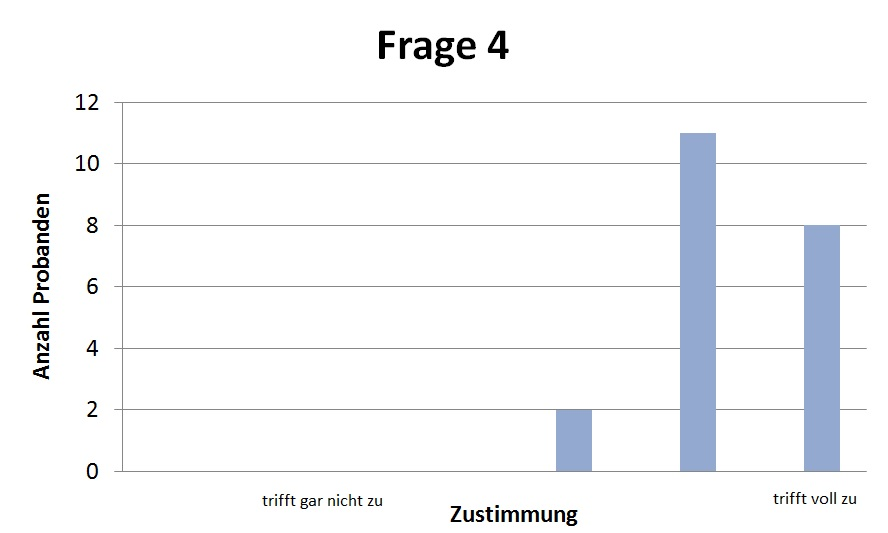
\includegraphics[width=0.7\linewidth]{img/Frage4}
\caption{Gesamtergebnis Frage 4}
\label{fig:Frage4}
\end{figure}\ \\
Diese Frage zielt auf den Gesamteindruck zum Design unseres Systems ab. Ein besonders ansprechendes Design erleichtert dem Nutzer die Bedienung, hat einen Wiedererkennungswert und bindet den Nutzer ans System. Die Ergebnisse der Evaluierung zeigen, dass die Webanwendung ofCourse bei den Testpersonen als sehr ansprechend empfunden wird.
\newpage
\subsection{Frage 5}
\begin{center}
	{\it Ich könnte mir vorstellen ofCourse in einem meiner Vereine/Sportgruppen/Lerngruppen/sonstige Gruppen zu nutzen.}
\end{center}
\begin{figure}[h]
\centering
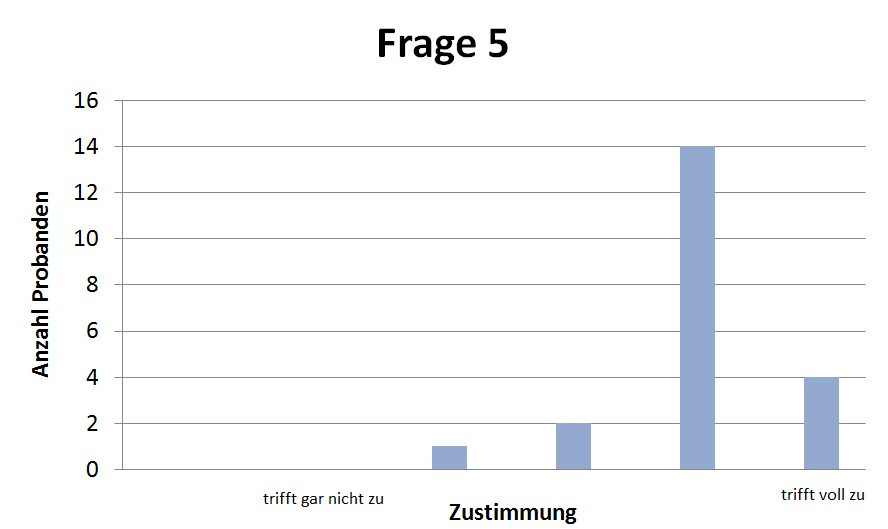
\includegraphics[width=0.7\linewidth]{img/Frage5}
\caption{Gesamtergebnis Frage 5}
\label{fig:Frage5}
\end{figure}
\ \\
Da unser System dafür gedacht ist, Veranstaltungen und deren Teilnahmen zu verwalten, zielt diese Frage darauf ab, ob Benutzer sich dafür entscheiden würden, dieses System in ihrem eigenen Verein(o.ä.) zu installieren bzw. als Vereinsmitglied(o.ä.) dieses System zu nutzen und damit zu arbeiten.\\
Wie unsere Erhebung zeigt, könnte sich eine Mehrheit vorstellen unser System in ihrem Vereinen zu nutzen.
\ \\

\newpage
\subsection{Bearbeitungszeit}
Für die Bearbeitung der Tests wurde von uns eine durchschnittliche Dauer von 10 - 15 Minuten veranschlagt. Im folgenden sind die 
von den Testpersonen gebrauchten Zeiten aufgeführt.\\

\begin{figure}[h]
\centering
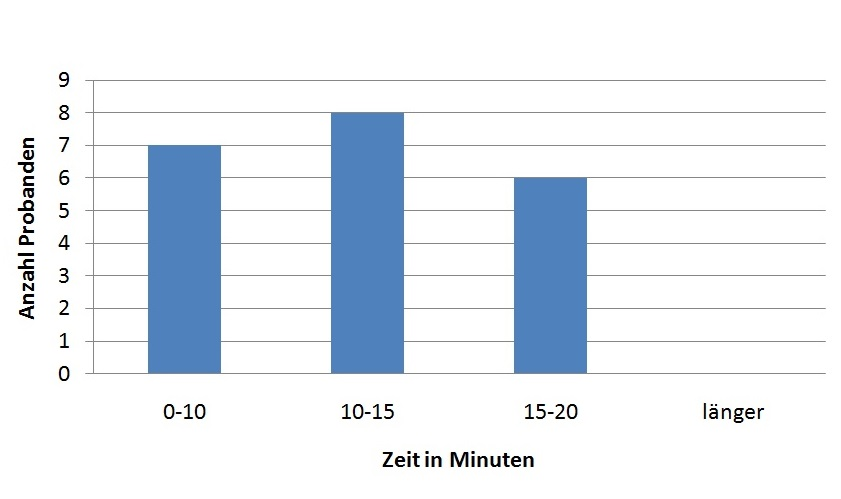
\includegraphics[width=0.7\linewidth]{img/Gesamtzeit}
\caption{Bearbeitungszeit der Tests}
\label{fig:Gesamtzeit}
\end{figure}
\ \\
Die Ergebnisse zeigen, dass eine Erledigung der von uns gestellten Aufgaben maximal 20 Minuten beansprucht, und das ohne als Nutzer jemals mit dem System in Kontakt gewesen zu sein. Das ist sehr nah an unserer Schätzung/Anforderung, zumal weniger als ein drittel der Probanden mehr als 15 Minuten benötigten. Bei wiederholter Nutzung ist also in Folge eines Lerneffekts von einer noch geringeren Dauer auszugehen. Aufgrund dieser Erkenntnisse lässt sich auf eine hohe Benutzbarkeit von ofCourse schließen.
\newpage



\subsection{Kritik/Anregungen/Verbessungsvorschläge}
In dem, beim Test verwendeten, Feedback-Bogen sind neben der oben aufgeführten Fragen noch weitere Unterpunkte zu finden. Unter anderem sollten die Probanden notieren, welche erledigte Aufgabe sie als besonders leicht und auch besonders schwer empfanden. Im Folgenden wird auf häufig Genanntes eingegangen.
\subsubsection{Kurssuche und -Anmeldung}
Zwei der sehr häufig genannten Aufgaben, welche als sehr leicht zu erledigen bezeichnet wurden, sind die Kurssuche als auch die Anmeldung zum Kurs. Dies konnten die Testpersonen der Gruppe eins schnell und ohne Komplikationen erledigen.
\subsubsection{Registrierung}
Die Registrierung stellte sich für viele Testpersonen als die schwierigste Aufgabe heraus. Es wurde zwar positiv genannt, dass die zu verwendende Seite sehr übersichtlich sei, jedoch war den Nutzern nicht klar, was die Sternchen hinter den einzelnen Feldertiteln bedeuten. Des weiteren und vermehrt bemängelt wurde außerdem die Wahl des Passworts. Dies war ein großes Hindernis bei der Registrierung, denn die Anforderungen an das zu wählende Passwort waren den Nutzern nicht klar. Für beide genannten Punkte wurden kurze Hilfetexte gewünscht.
\subsubsection{Design}
Vermehrt als sehr positiv bezeichnet, wurde die Struktur und das Design von ofCourse. Die Probanden lobten dessen Schlichtheit und Klarheit. Dieses erlaube eine intuitive Benutzung und sei außerdem sehr übersichtlich. Im Speziellen betont wurden außerdem die gut erkennbaren und farbigen Buttons, welche eine einfache Bedienung ermöglichen.
\subsubsection{Erfolgs- und Fehlermeldungen}
Beim Thema Erfolgs- und Fehlermeldungen zeigte sich ein klares Bedürfnis nach mehr Feedback. Mehr Meldungen sind ein häufig genanntes Stichwort der Fragebogen-Kategorie zu den gewünschten Änderungen. Konkret genannt wurde beispielsweise eine E-Mail-wurde-versand-Meldung bei der Registrierung und eine Erfolgsmeldung beim festlegen des Überziehungskredits.

\newpage
\section{Fazit}
Alles in einem betrachtet zeigt sich in den Ergebnissen unserer Evaluierung, dass ofCourse bereits ein sehr benutzerfreundliches System ist, welches sich, unter anderem, durch ein durchdachtes Design, leichte Bedienbarkeit und unkomplizierten Strukturen auszeichnet. Trotz der bereits vorhandenen Qualität, gibt es jedoch an manchen Stellen noch Bedarf zur Nachbesserung. So muss die Registrierungsseite beispielsweise bis zur endgültigen Systemabnahme noch etwas verständlicher gemacht, als auch noch diverse Fehler- und Erfolgsmeldungen im System eingebaut werden. Nach erfolgreichem Einbau des gewonnenen Feedbacks jedoch, steht der Nutzung des Systems jedoch nichts mehr entgegen, denn wie unter Anderem Abbildung 3.5 zeigt, können sich bereits jetzt viele Nutzer vorstellen, dieses System weitestgehend zu nutzen.